% Options for packages loaded elsewhere
% Options for packages loaded elsewhere
\PassOptionsToPackage{unicode}{hyperref}
\PassOptionsToPackage{hyphens}{url}
\PassOptionsToPackage{dvipsnames,svgnames,x11names}{xcolor}
%
\documentclass[
  letterpaper,
  DIV=11,
  numbers=noendperiod]{scrartcl}
\usepackage{xcolor}
\usepackage{amsmath,amssymb}
\setcounter{secnumdepth}{-\maxdimen} % remove section numbering
\usepackage{iftex}
\ifPDFTeX
  \usepackage[T1]{fontenc}
  \usepackage[utf8]{inputenc}
  \usepackage{textcomp} % provide euro and other symbols
\else % if luatex or xetex
  \usepackage{unicode-math} % this also loads fontspec
  \defaultfontfeatures{Scale=MatchLowercase}
  \defaultfontfeatures[\rmfamily]{Ligatures=TeX,Scale=1}
\fi
\usepackage{lmodern}
\ifPDFTeX\else
  % xetex/luatex font selection
\fi
% Use upquote if available, for straight quotes in verbatim environments
\IfFileExists{upquote.sty}{\usepackage{upquote}}{}
\IfFileExists{microtype.sty}{% use microtype if available
  \usepackage[]{microtype}
  \UseMicrotypeSet[protrusion]{basicmath} % disable protrusion for tt fonts
}{}
\makeatletter
\@ifundefined{KOMAClassName}{% if non-KOMA class
  \IfFileExists{parskip.sty}{%
    \usepackage{parskip}
  }{% else
    \setlength{\parindent}{0pt}
    \setlength{\parskip}{6pt plus 2pt minus 1pt}}
}{% if KOMA class
  \KOMAoptions{parskip=half}}
\makeatother
% Make \paragraph and \subparagraph free-standing
\makeatletter
\ifx\paragraph\undefined\else
  \let\oldparagraph\paragraph
  \renewcommand{\paragraph}{
    \@ifstar
      \xxxParagraphStar
      \xxxParagraphNoStar
  }
  \newcommand{\xxxParagraphStar}[1]{\oldparagraph*{#1}\mbox{}}
  \newcommand{\xxxParagraphNoStar}[1]{\oldparagraph{#1}\mbox{}}
\fi
\ifx\subparagraph\undefined\else
  \let\oldsubparagraph\subparagraph
  \renewcommand{\subparagraph}{
    \@ifstar
      \xxxSubParagraphStar
      \xxxSubParagraphNoStar
  }
  \newcommand{\xxxSubParagraphStar}[1]{\oldsubparagraph*{#1}\mbox{}}
  \newcommand{\xxxSubParagraphNoStar}[1]{\oldsubparagraph{#1}\mbox{}}
\fi
\makeatother

\usepackage{color}
\usepackage{fancyvrb}
\newcommand{\VerbBar}{|}
\newcommand{\VERB}{\Verb[commandchars=\\\{\}]}
\DefineVerbatimEnvironment{Highlighting}{Verbatim}{commandchars=\\\{\}}
% Add ',fontsize=\small' for more characters per line
\usepackage{framed}
\definecolor{shadecolor}{RGB}{241,243,245}
\newenvironment{Shaded}{\begin{snugshade}}{\end{snugshade}}
\newcommand{\AlertTok}[1]{\textcolor[rgb]{0.68,0.00,0.00}{#1}}
\newcommand{\AnnotationTok}[1]{\textcolor[rgb]{0.37,0.37,0.37}{#1}}
\newcommand{\AttributeTok}[1]{\textcolor[rgb]{0.40,0.45,0.13}{#1}}
\newcommand{\BaseNTok}[1]{\textcolor[rgb]{0.68,0.00,0.00}{#1}}
\newcommand{\BuiltInTok}[1]{\textcolor[rgb]{0.00,0.23,0.31}{#1}}
\newcommand{\CharTok}[1]{\textcolor[rgb]{0.13,0.47,0.30}{#1}}
\newcommand{\CommentTok}[1]{\textcolor[rgb]{0.37,0.37,0.37}{#1}}
\newcommand{\CommentVarTok}[1]{\textcolor[rgb]{0.37,0.37,0.37}{\textit{#1}}}
\newcommand{\ConstantTok}[1]{\textcolor[rgb]{0.56,0.35,0.01}{#1}}
\newcommand{\ControlFlowTok}[1]{\textcolor[rgb]{0.00,0.23,0.31}{\textbf{#1}}}
\newcommand{\DataTypeTok}[1]{\textcolor[rgb]{0.68,0.00,0.00}{#1}}
\newcommand{\DecValTok}[1]{\textcolor[rgb]{0.68,0.00,0.00}{#1}}
\newcommand{\DocumentationTok}[1]{\textcolor[rgb]{0.37,0.37,0.37}{\textit{#1}}}
\newcommand{\ErrorTok}[1]{\textcolor[rgb]{0.68,0.00,0.00}{#1}}
\newcommand{\ExtensionTok}[1]{\textcolor[rgb]{0.00,0.23,0.31}{#1}}
\newcommand{\FloatTok}[1]{\textcolor[rgb]{0.68,0.00,0.00}{#1}}
\newcommand{\FunctionTok}[1]{\textcolor[rgb]{0.28,0.35,0.67}{#1}}
\newcommand{\ImportTok}[1]{\textcolor[rgb]{0.00,0.46,0.62}{#1}}
\newcommand{\InformationTok}[1]{\textcolor[rgb]{0.37,0.37,0.37}{#1}}
\newcommand{\KeywordTok}[1]{\textcolor[rgb]{0.00,0.23,0.31}{\textbf{#1}}}
\newcommand{\NormalTok}[1]{\textcolor[rgb]{0.00,0.23,0.31}{#1}}
\newcommand{\OperatorTok}[1]{\textcolor[rgb]{0.37,0.37,0.37}{#1}}
\newcommand{\OtherTok}[1]{\textcolor[rgb]{0.00,0.23,0.31}{#1}}
\newcommand{\PreprocessorTok}[1]{\textcolor[rgb]{0.68,0.00,0.00}{#1}}
\newcommand{\RegionMarkerTok}[1]{\textcolor[rgb]{0.00,0.23,0.31}{#1}}
\newcommand{\SpecialCharTok}[1]{\textcolor[rgb]{0.37,0.37,0.37}{#1}}
\newcommand{\SpecialStringTok}[1]{\textcolor[rgb]{0.13,0.47,0.30}{#1}}
\newcommand{\StringTok}[1]{\textcolor[rgb]{0.13,0.47,0.30}{#1}}
\newcommand{\VariableTok}[1]{\textcolor[rgb]{0.07,0.07,0.07}{#1}}
\newcommand{\VerbatimStringTok}[1]{\textcolor[rgb]{0.13,0.47,0.30}{#1}}
\newcommand{\WarningTok}[1]{\textcolor[rgb]{0.37,0.37,0.37}{\textit{#1}}}

\usepackage{longtable,booktabs,array}
\newcounter{none} % for unnumbered tables
\usepackage{calc} % for calculating minipage widths
% Correct order of tables after \paragraph or \subparagraph
\usepackage{etoolbox}
\makeatletter
\patchcmd\longtable{\par}{\if@noskipsec\mbox{}\fi\par}{}{}
\makeatother
% Allow footnotes in longtable head/foot
\IfFileExists{footnotehyper.sty}{\usepackage{footnotehyper}}{\usepackage{footnote}}
\makesavenoteenv{longtable}
\usepackage{graphicx}
\makeatletter
\newsavebox\pandoc@box
\newcommand*\pandocbounded[1]{% scales image to fit in text height/width
  \sbox\pandoc@box{#1}%
  \Gscale@div\@tempa{\textheight}{\dimexpr\ht\pandoc@box+\dp\pandoc@box\relax}%
  \Gscale@div\@tempb{\linewidth}{\wd\pandoc@box}%
  \ifdim\@tempb\p@<\@tempa\p@\let\@tempa\@tempb\fi% select the smaller of both
  \ifdim\@tempa\p@<\p@\scalebox{\@tempa}{\usebox\pandoc@box}%
  \else\usebox{\pandoc@box}%
  \fi%
}
% Set default figure placement to htbp
\def\fps@figure{htbp}
\makeatother





\setlength{\emergencystretch}{3em} % prevent overfull lines

\providecommand{\tightlist}{%
  \setlength{\itemsep}{0pt}\setlength{\parskip}{0pt}}



 


\KOMAoption{captions}{tableheading}
\makeatletter
\@ifpackageloaded{caption}{}{\usepackage{caption}}
\AtBeginDocument{%
\ifdefined\contentsname
  \renewcommand*\contentsname{Table of contents}
\else
  \newcommand\contentsname{Table of contents}
\fi
\ifdefined\listfigurename
  \renewcommand*\listfigurename{List of Figures}
\else
  \newcommand\listfigurename{List of Figures}
\fi
\ifdefined\listtablename
  \renewcommand*\listtablename{List of Tables}
\else
  \newcommand\listtablename{List of Tables}
\fi
\ifdefined\figurename
  \renewcommand*\figurename{Figure}
\else
  \newcommand\figurename{Figure}
\fi
\ifdefined\tablename
  \renewcommand*\tablename{Table}
\else
  \newcommand\tablename{Table}
\fi
}
\@ifpackageloaded{float}{}{\usepackage{float}}
\floatstyle{ruled}
\@ifundefined{c@chapter}{\newfloat{codelisting}{h}{lop}}{\newfloat{codelisting}{h}{lop}[chapter]}
\floatname{codelisting}{Listing}
\newcommand*\listoflistings{\listof{codelisting}{List of Listings}}
\makeatother
\makeatletter
\makeatother
\makeatletter
\@ifpackageloaded{caption}{}{\usepackage{caption}}
\@ifpackageloaded{subcaption}{}{\usepackage{subcaption}}
\makeatother
\usepackage{bookmark}
\IfFileExists{xurl.sty}{\usepackage{xurl}}{} % add URL line breaks if available
\urlstyle{same}
\hypersetup{
  pdftitle={Arielle Camera Trap Workflow},
  pdfauthor={Arielle Escareno; Charles Lehnen},
  colorlinks=true,
  linkcolor={blue},
  filecolor={Maroon},
  citecolor={Blue},
  urlcolor={Blue},
  pdfcreator={LaTeX via pandoc}}


\title{Arielle Camera Trap Workflow}
\author{Arielle Escareno \and Charles Lehnen}
\date{}
\begin{document}
\maketitle


\section{Arielle's Camera Trap
Workflow}\label{arielles-camera-trap-workflow}

\subsection{A Guide To Classifying Camera Trap
Images}\label{a-guide-to-classifying-camera-trap-images}

\subsection{Project Overview}\label{project-overview}

This project investigates whether introduced Giant Galápagos tortoises
(\emph{Chelonoidis hoodensis}) and Santa Fé iguanas (\emph{Conolophus
pallidus}) share overlapping habitat on Santa Fé Island in the Galápagos
Archipelago, or actively avoid direct competition with one another.
Using five Reconyx Hyperfire 2 camera traps placed across the island
from July 2023 to May 2025, I classified hundreds of camera trap images
to examine when and where each species was detected. Raw images were
processed using an automated detection model (MegaDetector) to identify
which images contained animals, and were then manually classified using
a custom Python-based tool built by my mentor, Charles Lehnen. My
findings suggest that while tortoises and iguanas were rarely
photographed together and tended to favor different camera trap sites,
both species were active during similar times of day, pointing to
spatial rather than temporal avoidance between the two species. This
site walks through the full technical process behind my analysis, from
setting up the environment to building the final figures.

\subsection{Background}\label{background}

Santa Fé Island is a small, remote island in the Galápagos Archipelago
of Ecuador.

\begin{center}
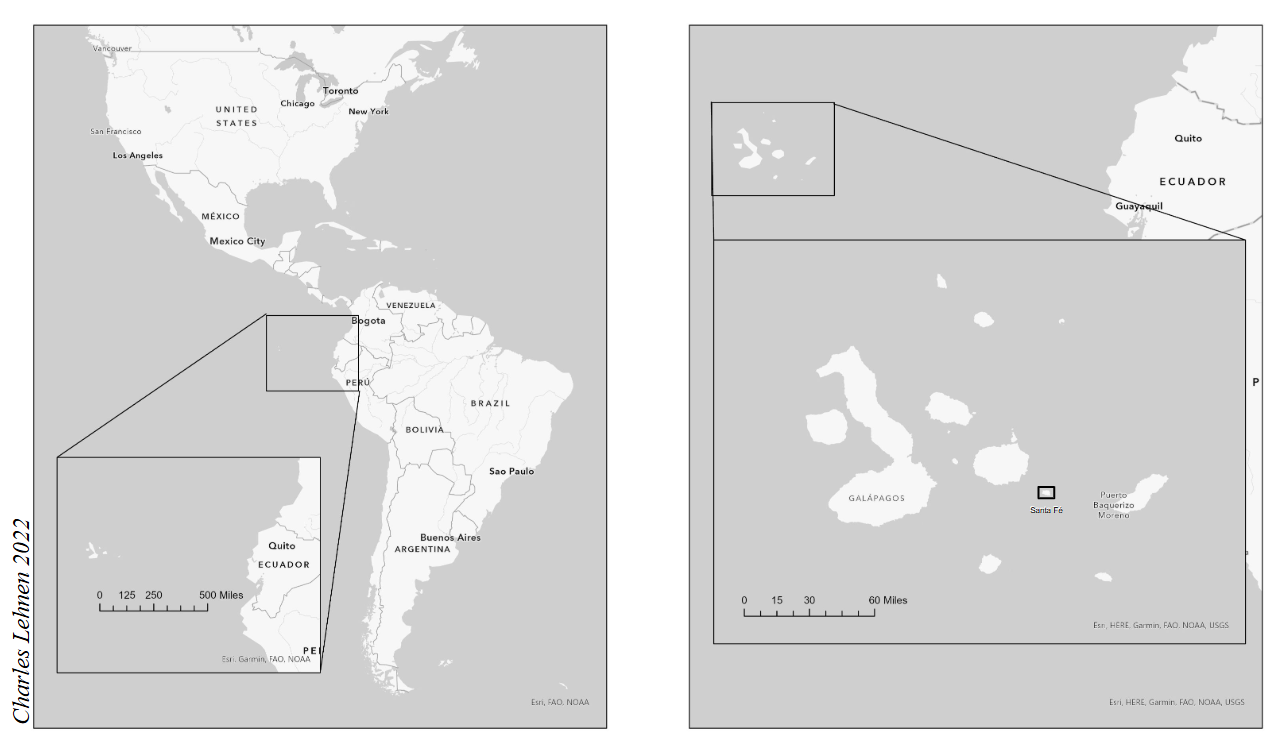
\includegraphics[width=7.76042in,height=\textheight,keepaspectratio]{images/paste-2.png}
\end{center}

\begin{itemize}
\tightlist
\item
  The Galápagos Islands are home to the endemic Galápagos iguanas and
  Galápagos tortoises.
\item
  Santa Fé Island is a small, remote island in the Galápagos Archipelago
  of Ecuador. It is home to the endemic Santa Fé land iguana
  (\emph{Conolophus pallidus}), but its native tortoise species
  (\emph{Chelonoidis indet.}) went extinct in the mid-1800s, largely due
  to hunting by sailors and whalers passing through the islands at the
  time.
\item
  Because no hybrids or even genetic samples of the original species
  survived, a closely related tortoise species (\emph{Chelonoidis
  hoodensis}) was introduced to the island starting in 2015 to help
  restore its ecological balance.
\item
  The Santa Fé land iguana, meanwhile, remained on the island throughout
  this time and was never displaced.
\item
  Because these species share the same environment, there may be spatial
  overlap or active avoidance between them.
\end{itemize}

\subsection{Tools Used}\label{tools-used}

\begin{itemize}
\tightlist
\item
  Positron (IDE)
\item
  Python 3.11
\item
  GitHub / GitHub Desktop
\item
  MegaDetector (AI detection model)
\item
  R (for data analysis and figures)
\item
  Markdown
\end{itemize}

\subsection{Learning GitHub and
Markdown}\label{learning-github-and-markdown}

Before starting the actual research project, my mentor introduced me to
GitHub and Markdown on my first day. GitHub is a platform used to store
code and track changes on a project over time, and Markdown is a simple
formatting language used to write styled text that is then converted
into HTML. To practice, I created a test README file written in Markdown
which was themed around SpongeBob just to get comfortable with the
syntax before using it on anything that mattered for my actual research.
I used a cheat sheet located on Charles Lehnen's website. This first day
is also where I learned the core Git vocabulary I'd use throughout the
rest of the project:

\begin{itemize}
\tightlist
\item
  \textbf{Commit} -- saving your changes, along with a short message
  describing what you changed
\item
  \textbf{Push} -- sending your committed changes up to GitHub, so
  they're saved online
\item
  \textbf{Pull} -- downloading any new changes from GitHub down to your
  own computer
\item
  \textbf{Fetch} -- checking GitHub for new changes Learning these
  basics early made the rest of the project much smoother, since I
  already understood how to save and track my work before I started
  making classifications.
\end{itemize}

\subsection{Step 1: Setting Up the
Environment}\label{step-1-setting-up-the-environment}

I had to download an IDE (Integrated Development Environment) to write
and run my code, so I used Positron. IDEs are what coders use to write,
test, and debug code. Other IDEs include RStudio, which is built
specifically to run R code. Positron, on the other hand, was built to
support both R and Python from the ground up, and since it's a fork of
VSCode, it can be made to run many other languages too.

\begin{itemize}
\tightlist
\item
  In order to run the classification GUI tool Charles built, I needed
  Python installed on my computer. Since my MacBook is from early 2015,
  I had to install an older, compatible version of Python using my Mac
  terminal.
\item
  I also had to set up a virtual environment (venv). A venv is like a
  boxed-up workspace that only contains a specific Python version and
  its dependencies, kept separate from anything else installed on the
  computer. I created mine using the terminal:
\end{itemize}

\begin{Shaded}
\begin{Highlighting}[]
\ExtensionTok{python3.11} \AttributeTok{{-}m}\NormalTok{ venv venv}
\BuiltInTok{source}\NormalTok{ venv/bin/activate}
\end{Highlighting}
\end{Shaded}

After that, I installed all the required dependencies (external code
libraries the project needed) so Python could actually run the tool:

\begin{Shaded}
\begin{Highlighting}[]
\ExtensionTok{pip}\NormalTok{ install }\AttributeTok{{-}r}\NormalTok{ requirements.txt}
\end{Highlighting}
\end{Shaded}

\subsection{Step 2: Running Unsupervised
Detection}\label{step-2-running-unsupervised-detection}

\begin{itemize}
\tightlist
\item
  MegaDetector is an open-source AI tool used to detect animals, humans,
  and vehicles in camera trap images. It scans through thousands of
  photos and filters out the blank ones automatically. MegaDetector
  assigns a confidence score to each detection, and the user chooses how
  confident the AI needs to be before counting something as a real
  detection. In my case, I was looking specifically for animals.
\item
  Running `capture\_images.py' starts this process automatically across
  all your images:
\end{itemize}

\begin{Shaded}
\begin{Highlighting}[]
\ExtensionTok{python3}\NormalTok{ code/capture\_images.py}
\end{Highlighting}
\end{Shaded}

\begin{itemize}
\tightlist
\item
  This produces outputs: bounding box images, cropped images (close ups
  of just the animals), and a `metadata.csv' file summarizing details
  like date, time, and camera location for each detection.
\end{itemize}

\subsection{Step 3: Manual
Classification}\label{step-3-manual-classification}

A GUI (Graphical User Interface) is a visual way to interact with a
program. Instead of writing code, you click or tap buttons. The image
classification tool I used was built by Charles Lehnen:
\href{https://github.com/CharlesLehnen/camera_trap_analysis}{view his
repository here}.
\pandocbounded{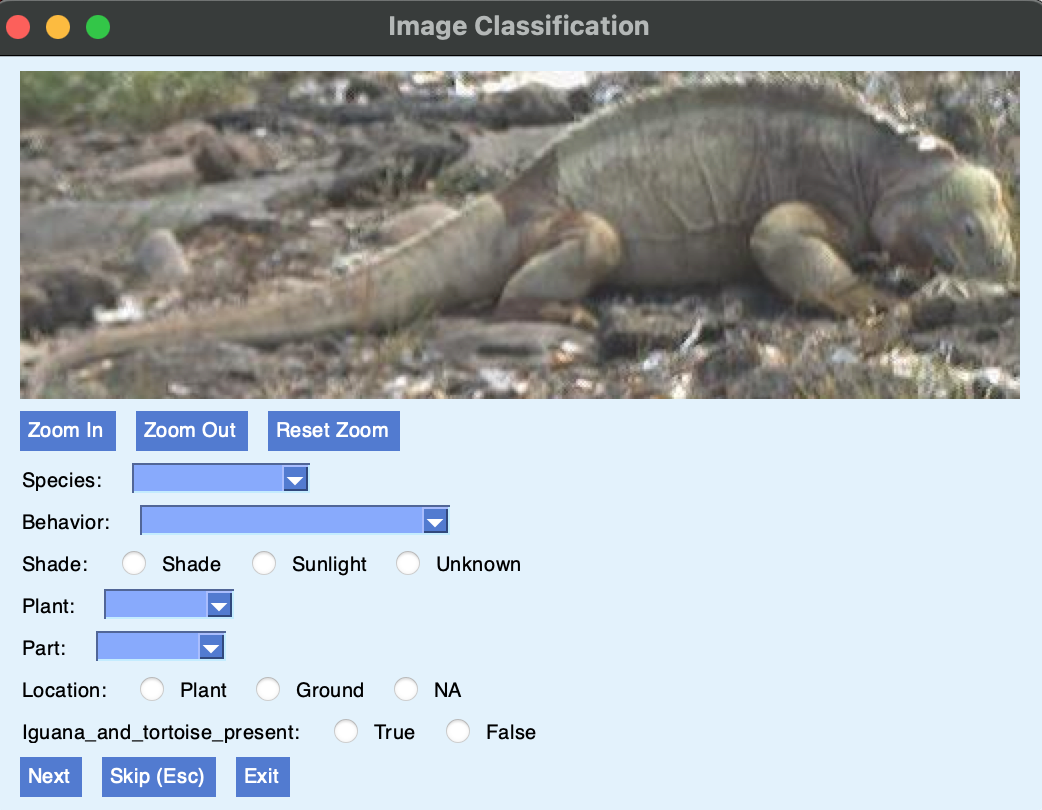
\includegraphics[keepaspectratio,alt={Image Classification GUI}]{Imagesss/image_class.png}}
The fields I classified for each image were: Species, Behavior, Shade,
Plant, Part, Location, and Iguana\_and\_tortoise\_present (True/False).

\begin{figure}[H]

{\centering \pandocbounded{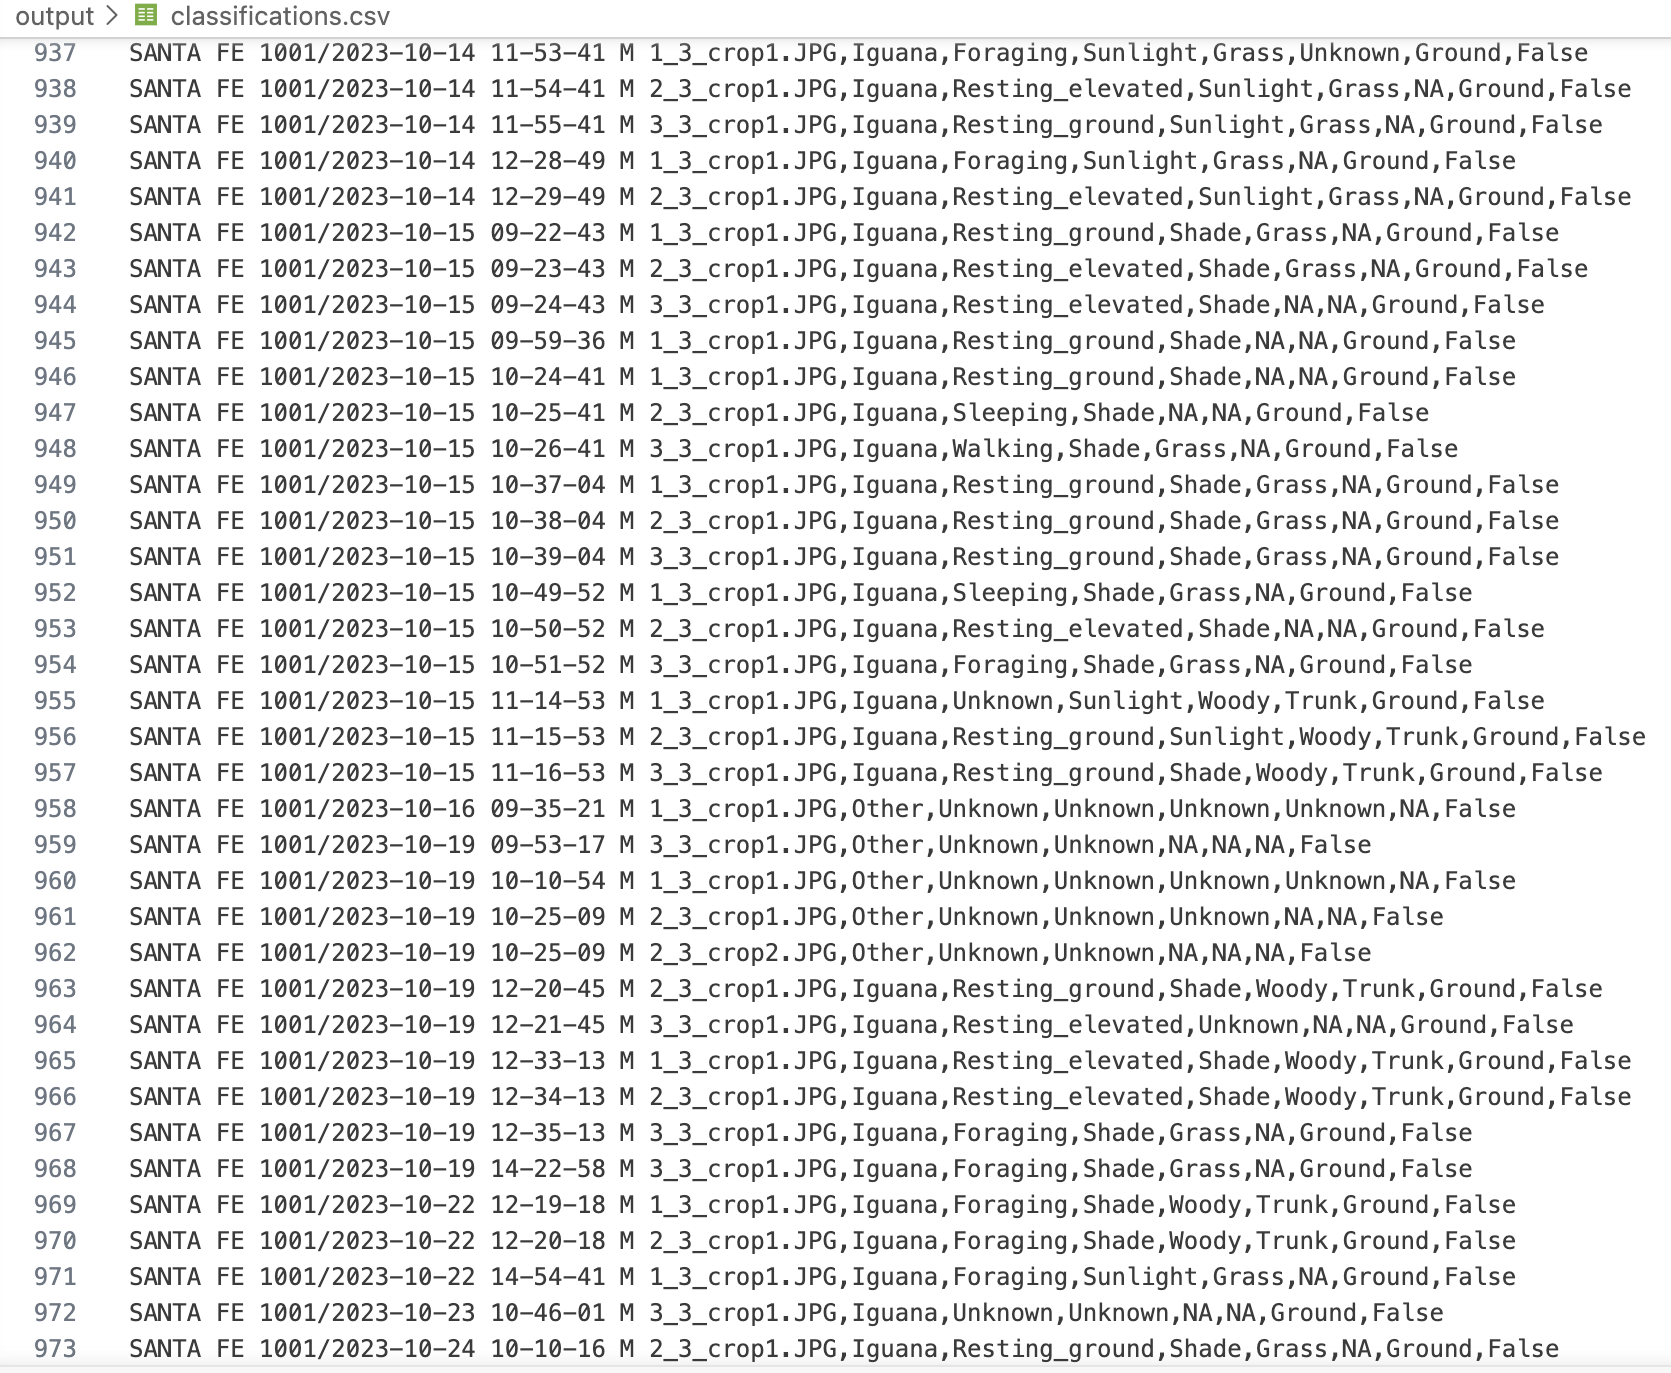
\includegraphics[keepaspectratio]{Imagesss/classificationss.png}}

}

\caption{My classifications viewed as a text file}

\end{figure}%

The GUI lets you classify using either keyboard shortcuts (faster, once
you know the categories) or dropdown/radio buttons (slower, but more
visual).

\begin{Shaded}
\begin{Highlighting}[]
\ExtensionTok{python3}\NormalTok{ code/image\_classification.py}
\end{Highlighting}
\end{Shaded}

\subsection{Step 4: Extracting Site and Time-of-Day
Data}\label{step-4-extracting-site-and-time-of-day-data}

Rather than manually recording which camera took each photo or what time
of day it was taken, this information was pulled directly from each
image's existing metadata.

\subsection{Step 5: Analyzing the Data in
R}\label{step-5-analyzing-the-data-in-r}

I used R to read in my finished `classifications.csv' file and calculate
the patterns behind my results: how often each species appeared
together, how their detections were distributed across camera sites, and
how their activity compared across different times of day. Using the
\texttt{ggplot2} package, four main figures were built from this data:

\begin{itemize}
\tightlist
\item
  A bar chart showing how rarely tortoises and iguanas were photographed
  together
\item
  A chart comparing where each species was detected across camera sites
\item
  A chart comparing each species' activity levels across different times
  of day
\item
  A heatmap showing which species was detected more often at each camera
  site during each time of day
\item
\end{itemize}

\subsection{Building the Figures:
species\_interactions.qmd}\label{building-the-figures-species_interactions.qmd}

All of my data analysis and figure building was done in a separate
Quarto file called `species\_interactions.qmd', using R. This file reads
in my finished `classifications.csv', processes it, and generates each
of the plots used in my results.

Here are the figures built, along with the code used to generate each
one:

\subsubsection{Clearing environment to have a clean
slate}\label{clearing-environment-to-have-a-clean-slate}

\begin{Shaded}
\begin{Highlighting}[]
\FunctionTok{rm}\NormalTok{(}\AttributeTok{list =} \FunctionTok{ls}\NormalTok{())}
\end{Highlighting}
\end{Shaded}

\subsubsection{Loading in the packages we
need}\label{loading-in-the-packages-we-need}

\begin{Shaded}
\begin{Highlighting}[]
\FunctionTok{library}\NormalTok{(readr) }
\FunctionTok{library}\NormalTok{(dplyr)}
\FunctionTok{library}\NormalTok{(ggplot2)}
\FunctionTok{library}\NormalTok{(janitor)}
\FunctionTok{library}\NormalTok{(stringr)}
\FunctionTok{library}\NormalTok{(lubridate)}
\FunctionTok{library}\NormalTok{(ggalluvial) }\CommentTok{\# for the alluvial plot}
\FunctionTok{library}\NormalTok{(webr) }\CommentTok{\# for the stacked donut plot}
\end{Highlighting}
\end{Shaded}

\subsubsection{Setting output folder for my
plots}\label{setting-output-folder-for-my-plots}

\begin{Shaded}
\begin{Highlighting}[]
\CommentTok{\# Output folder}
\FunctionTok{dir.create}\NormalTok{(}\StringTok{"../output/r\_analysis"}\NormalTok{, }\AttributeTok{showWarnings =} \ConstantTok{FALSE}\NormalTok{, }\AttributeTok{recursive =} \ConstantTok{TRUE}\NormalTok{)}
\end{Highlighting}
\end{Shaded}

\subsubsection{Loading in our data}\label{loading-in-our-data}

\begin{Shaded}
\begin{Highlighting}[]
\CommentTok{\# Dealing with different OSs }
\NormalTok{read\_first\_existing }\OtherTok{\textless{}{-}} \ControlFlowTok{function}\NormalTok{(candidates) \{}
  \ControlFlowTok{for}\NormalTok{ (path }\ControlFlowTok{in}\NormalTok{ candidates) \{}
    \ControlFlowTok{if}\NormalTok{ (}\FunctionTok{file.exists}\NormalTok{(path)) \{}
      \FunctionTok{return}\NormalTok{(}\FunctionTok{read.csv}\NormalTok{(}\AttributeTok{file =}\NormalTok{ path))}
\NormalTok{    \}}
\NormalTok{  \}}
  \FunctionTok{stop}\NormalTok{(}\StringTok{"None of the candidate paths exist: "}\NormalTok{, }\FunctionTok{paste}\NormalTok{(candidates, }\AttributeTok{collapse =} \StringTok{", "}\NormalTok{))}
\NormalTok{\}}

\NormalTok{dfclassifications }\OtherTok{\textless{}{-}} \FunctionTok{read\_first\_existing}\NormalTok{(}\FunctionTok{c}\NormalTok{(}
  \StringTok{"../output/classifications.csv"}\NormalTok{,}
  \StringTok{"/output/classifications.csv"}\NormalTok{,}
  \StringTok{"output/classifications.csv"}
\NormalTok{))}
\NormalTok{dfclassifications\_random }\OtherTok{\textless{}{-}} \FunctionTok{read\_first\_existing}\NormalTok{(}\FunctionTok{c}\NormalTok{(}
  \StringTok{"../output/classifications\_random\_order.csv"}\NormalTok{,}
  \StringTok{"/output/classifications\_random\_order.csv"}\NormalTok{,}
  \StringTok{"output/classifications\_random\_order.csv"}
\NormalTok{))}
\NormalTok{dfmetadata }\OtherTok{\textless{}{-}} \FunctionTok{read\_first\_existing}\NormalTok{(}\FunctionTok{c}\NormalTok{(}
  \StringTok{"../output/metadata/metadata.csv"}\NormalTok{,}
  \StringTok{"/output/metadata/metadata.csv"}\NormalTok{,}
  \StringTok{"output/metadata/metadata.csv"}
\NormalTok{))}
\end{Highlighting}
\end{Shaded}

\subsubsection{Exploring our data}\label{exploring-our-data}

\begin{Shaded}
\begin{Highlighting}[]
\FunctionTok{head}\NormalTok{(dfclassifications)}
\end{Highlighting}
\end{Shaded}

\begin{verbatim}
                                              Image  Species         Behavior
1        2023-08-08 08-15-11 M 1_3_crop1_buf100.JPG Tortoise          Walking
2        2023-08-12 13-19-06 M 3_3_crop1_buf100.JPG Tortoise         Foraging
3        2023-08-20 07-46-06 M 1_3_crop1_buf100.JPG Tortoise          Walking
4 SANTA FE 1001/2023-07-28 09-55-00 M 1_3_crop1.JPG   Iguana Resting_elevated
5 SANTA FE 1001/2023-07-28 09-57-00 M 3_3_crop1.JPG   Iguana   Resting_ground
6 SANTA FE 1001/2023-07-28 12-02-40 M 1_3_crop1.JPG   Iguana         Foraging
     Shade Plant  Part Location Iguana_and_tortoise_present
1 Sunlight  <NA>  <NA>     <NA>                            
2    Shade Grass Trunk   Ground                            
3 Sunlight  <NA>  <NA>   Ground                            
4    Shade  <NA>  <NA>   Ground                       False
5    Shade  <NA>  <NA>   Ground                       False
6    Shade  <NA>  <NA>     <NA>                       False
\end{verbatim}

\begin{Shaded}
\begin{Highlighting}[]
\FunctionTok{summary}\NormalTok{(dfclassifications)}
\end{Highlighting}
\end{Shaded}

\begin{verbatim}
       Image           Species          Behavior          Shade     
 Length   :1155   Length   :1155   Length   :1155   Length   :1155  
 N.unique : 498   N.unique :   7   N.unique :  12   N.unique :   5  
 N.blank  :   0   N.blank  :   0   N.blank  :   0   N.blank  :   0  
 Min.nchar:   6   Min.nchar:   4   Min.nchar:   5   Min.nchar:   5  
 Max.nchar:  49   Max.nchar:  11   Max.nchar:  22   Max.nchar:   8  
                                                                    
       Plant             Part           Location    Iguana_and_tortoise_present
 Length   :1155   Length   :1155   Length   :1155   Length   :1155             
 N.unique :   4   N.unique :   5   N.unique :   4   N.unique :   5             
 N.blank  :   0   N.blank  :   0   N.blank  :   0   N.blank  :  13             
 Min.nchar:   5   Min.nchar:   4   Min.nchar:   5   Min.nchar:   0             
 Max.nchar:   7   Max.nchar:   7   Max.nchar:   7   Max.nchar:  54             
 NAs      : 387   NAs      : 818   NAs      : 206                              
\end{verbatim}

\begin{Shaded}
\begin{Highlighting}[]
\FunctionTok{str}\NormalTok{(dfclassifications)}
\end{Highlighting}
\end{Shaded}

\begin{verbatim}
'data.frame':   1155 obs. of  8 variables:
 $ Image                      : chr  "2023-08-08 08-15-11 M 1_3_crop1_buf100.JPG" "2023-08-12 13-19-06 M 3_3_crop1_buf100.JPG" "2023-08-20 07-46-06 M 1_3_crop1_buf100.JPG" "SANTA FE 1001/2023-07-28 09-55-00 M 1_3_crop1.JPG" ...
 $ Species                    : chr  "Tortoise" "Tortoise" "Tortoise" "Iguana" ...
 $ Behavior                   : chr  "Walking" "Foraging" "Walking" "Resting_elevated" ...
 $ Shade                      : chr  "Sunlight" "Shade" "Sunlight" "Shade" ...
 $ Plant                      : chr  NA "Grass" NA NA ...
 $ Part                       : chr  NA "Trunk" NA NA ...
 $ Location                   : chr  NA "Ground" "Ground" "Ground" ...
 $ Iguana_and_tortoise_present: chr  "" "" "" "False" ...
\end{verbatim}

\subsubsection{Cleaning our data}\label{cleaning-our-data}

\begin{Shaded}
\begin{Highlighting}[]
\NormalTok{dfclassifications\_clean }\OtherTok{\textless{}{-}}\NormalTok{ dfclassifications }\SpecialCharTok{\%\textgreater{}\%}
  \FunctionTok{clean\_names}\NormalTok{() }\SpecialCharTok{\%\textgreater{}\%}
  \FunctionTok{rename\_with}\NormalTok{(}\SpecialCharTok{\textasciitilde{}} \StringTok{"species"}\NormalTok{, }\FunctionTok{ends\_with}\NormalTok{(}\StringTok{"species"}\NormalTok{)) }\SpecialCharTok{\%\textgreater{}\%}
  \FunctionTok{filter}\NormalTok{(species }\SpecialCharTok{!=} \StringTok{""}\NormalTok{) }\SpecialCharTok{\%\textgreater{}\%}
  \CommentTok{\# If a crop was labelled out of the buffered folder it carries a \_buf100 suffix that the metadata doesn\textquotesingle{}t have. drop it so the two match.}
  \FunctionTok{mutate}\NormalTok{(}\AttributeTok{crop\_path =} \FunctionTok{str\_replace}\NormalTok{(image, }\StringTok{"\_buf}\SpecialCharTok{\textbackslash{}\textbackslash{}}\StringTok{d+(}\SpecialCharTok{\textbackslash{}\textbackslash{}}\StringTok{.[\^{}.]+)$"}\NormalTok{, }\StringTok{"}\SpecialCharTok{\textbackslash{}\textbackslash{}}\StringTok{1"}\NormalTok{)) }\SpecialCharTok{\%\textgreater{}\%}
  \FunctionTok{mutate}\NormalTok{(}\AttributeTok{crop\_path =} \FunctionTok{str\_replace}\NormalTok{(crop\_path, }\StringTok{"\^{}}\SpecialCharTok{\textbackslash{}\textbackslash{}}\StringTok{./"}\NormalTok{, }\StringTok{""}\NormalTok{))}

\NormalTok{dfmetadata\_clean }\OtherTok{\textless{}{-}}\NormalTok{ dfmetadata }\SpecialCharTok{\%\textgreater{}\%}
  \FunctionTok{clean\_names}\NormalTok{() }\SpecialCharTok{\%\textgreater{}\%}

  \CommentTok{\# get column name formats to match}
  \FunctionTok{mutate}\NormalTok{(}\AttributeTok{crop\_path =} \FunctionTok{str\_remove}\NormalTok{(cropped\_image, }\StringTok{"\^{}.*output/cropped/"}\NormalTok{)) }\SpecialCharTok{\%\textgreater{}\%}
  \FunctionTok{mutate}\NormalTok{(}
    \AttributeTok{first\_seg =} \FunctionTok{str\_replace}\NormalTok{(subfolder, }\StringTok{"[/}\SpecialCharTok{\textbackslash{}\textbackslash{}\textbackslash{}\textbackslash{}}\StringTok{].*$"}\NormalTok{, }\StringTok{""}\NormalTok{), }
    \AttributeTok{cam\_id    =} \FunctionTok{str\_extract}\NormalTok{(first\_seg, }\StringTok{"}\SpecialCharTok{\textbackslash{}\textbackslash{}}\StringTok{d\{3,\}"}\NormalTok{),}
    \AttributeTok{camera\_trap\_name =} \FunctionTok{if\_else}\NormalTok{(}\FunctionTok{is.na}\NormalTok{(cam\_id), }\StringTok{"000"}\NormalTok{, cam\_id)}
\NormalTok{  ) }\SpecialCharTok{\%\textgreater{}\%}
  
  \FunctionTok{mutate}\NormalTok{(}
    \AttributeTok{dt   =} \FunctionTok{parse\_date\_time}\NormalTok{(date\_time\_original, }\AttributeTok{orders =} \StringTok{"Y:m:d H:M:S"}\NormalTok{),}
    \AttributeTok{date =} \FunctionTok{as\_date}\NormalTok{(dt),}
    \AttributeTok{hour =} \FunctionTok{hour}\NormalTok{(dt)}
\NormalTok{  ) }\SpecialCharTok{\%\textgreater{}\%}

  \CommentTok{\# Santa Fe sits on the equator, so daylight is roughly 06:00{-}18:00 year round}
  \FunctionTok{mutate}\NormalTok{(}\AttributeTok{time\_of\_day =} \FunctionTok{case\_when}\NormalTok{(}
\NormalTok{    hour }\SpecialCharTok{\textgreater{}=} \DecValTok{6}  \SpecialCharTok{\&}\NormalTok{ hour }\SpecialCharTok{\textless{}} \DecValTok{11} \SpecialCharTok{\textasciitilde{}} \StringTok{"Morning"}\NormalTok{,}
\NormalTok{    hour }\SpecialCharTok{\textgreater{}=} \DecValTok{11} \SpecialCharTok{\&}\NormalTok{ hour }\SpecialCharTok{\textless{}} \DecValTok{15} \SpecialCharTok{\textasciitilde{}} \StringTok{"Midday"}\NormalTok{,}
\NormalTok{    hour }\SpecialCharTok{\textgreater{}=} \DecValTok{15} \SpecialCharTok{\&}\NormalTok{ hour }\SpecialCharTok{\textless{}} \DecValTok{18} \SpecialCharTok{\textasciitilde{}} \StringTok{"Afternoon"}\NormalTok{,}
    \ConstantTok{TRUE} \SpecialCharTok{\textasciitilde{}} \StringTok{"Night"}
\NormalTok{  )) }\SpecialCharTok{\%\textgreater{}\%}
  \FunctionTok{mutate}\NormalTok{(}\AttributeTok{time\_of\_day =} \FunctionTok{factor}\NormalTok{(time\_of\_day,}
                              \AttributeTok{levels =} \FunctionTok{c}\NormalTok{(}\StringTok{"Morning"}\NormalTok{, }\StringTok{"Midday"}\NormalTok{, }\StringTok{"Afternoon"}\NormalTok{, }\StringTok{"Night"}\NormalTok{))) }\SpecialCharTok{\%\textgreater{}\%}
  \CommentTok{\# select only the columns we need}
  \FunctionTok{select}\NormalTok{(subfolder, original\_image, crop\_path, camera\_trap\_name,}
\NormalTok{         dt, date, hour, time\_of\_day, confidence)}


\FunctionTok{summary}\NormalTok{(dfmetadata\_clean)}
\end{Highlighting}
\end{Shaded}

\begin{verbatim}
     subfolder      original_image     crop_path     camera_trap_name
 Length   :7850   Length   :7850   Length   :7850   Length   :7850   
 N.unique :  10   N.unique :5613   N.unique :5936   N.unique :   6   
 N.blank  :   0   N.blank  :   0   N.blank  :   0   N.blank  :   0   
 Min.nchar:   8   Min.nchar:  38   Min.nchar:  44   Min.nchar:   3   
 Max.nchar:  26   Max.nchar:  43   Max.nchar:  49   Max.nchar:   4   
                                                                     
                                                                     
       dt                           date                 hour      
 Min.   :2023-07-24 16:38:47   Min.   :2023-07-24   Min.   : 6.00  
 1st Qu.:2023-10-02 16:38:40   1st Qu.:2023-10-02   1st Qu.:10.00  
 Median :2023-12-23 15:14:53   Median :2023-12-23   Median :12.00  
 Mean   :2024-01-05 12:38:48   Mean   :2024-01-05   Mean   :11.49  
 3rd Qu.:2024-03-06 12:38:45   3rd Qu.:2024-03-06   3rd Qu.:13.00  
 Max.   :2025-05-02 12:16:38   Max.   :2025-05-02   Max.   :18.00  
 NAs    :484                   NAs    :484          NAs    :484    
    time_of_day     confidence    
 Morning  :2483   Min.   :0.5000  
 Midday   :4080   1st Qu.:0.6603  
 Afternoon: 797   Median :0.7770  
 Night    : 490   Mean   :0.7713  
                  3rd Qu.:0.8990  
                  Max.   :0.9840  
                                  
\end{verbatim}

\subsubsection{Joining my data with the
metadata}\label{joining-my-data-with-the-metadata}

\begin{Shaded}
\begin{Highlighting}[]
\CommentTok{\# inner\_join because a crop is only useful here if we both detected AND labelled it.}
\NormalTok{dfjoined }\OtherTok{\textless{}{-}}\NormalTok{ dfclassifications\_clean }\SpecialCharTok{\%\textgreater{}\%}
  \FunctionTok{inner\_join}\NormalTok{(dfmetadata\_clean, }\AttributeTok{by =} \StringTok{"crop\_path"}\NormalTok{)}

\CommentTok{\# Just our two focal species}
\NormalTok{dffocal }\OtherTok{\textless{}{-}}\NormalTok{ dfjoined }\SpecialCharTok{\%\textgreater{}\%}
  \FunctionTok{filter}\NormalTok{(species }\SpecialCharTok{\%in\%} \FunctionTok{c}\NormalTok{(}\StringTok{"Tortoise"}\NormalTok{, }\StringTok{"Iguana"}\NormalTok{))}

\FunctionTok{nrow}\NormalTok{(dfclassifications\_clean)}
\end{Highlighting}
\end{Shaded}

\begin{verbatim}
[1] 1155
\end{verbatim}

\begin{Shaded}
\begin{Highlighting}[]
\FunctionTok{nrow}\NormalTok{(dfjoined)}
\end{Highlighting}
\end{Shaded}

\begin{verbatim}
[1] 1142
\end{verbatim}

\subsubsection{Co-occurrence Bar Chart}\label{co-occurrence-bar-chart}

\begin{Shaded}
\begin{Highlighting}[]
\NormalTok{dfphoto\_focal }\SpecialCharTok{\%\textgreater{}\%}
  \FunctionTok{ggplot}\NormalTok{(}\FunctionTok{aes}\NormalTok{(}\AttributeTok{x =}\NormalTok{ composition)) }\SpecialCharTok{+}
  \FunctionTok{geom\_bar}\NormalTok{(}\AttributeTok{fill =} \StringTok{"\#9a0101"}\NormalTok{, }\AttributeTok{alpha =} \FloatTok{0.8}\NormalTok{) }\SpecialCharTok{+}
  \FunctionTok{labs}\NormalTok{(}\AttributeTok{title =} \StringTok{"Tortoises and Iguanas Rarely Share a Photo"}\NormalTok{,}
       \AttributeTok{x =} \StringTok{"What was in the photo"}\NormalTok{, }\AttributeTok{y =} \StringTok{"Number of photos"}\NormalTok{) }\SpecialCharTok{+}
  \FunctionTok{theme\_bw}\NormalTok{() }\SpecialCharTok{+}
  \FunctionTok{theme}\NormalTok{(}\AttributeTok{plot.title =} \FunctionTok{element\_text}\NormalTok{(}\AttributeTok{hjust =} \FloatTok{0.5}\NormalTok{))}

\FunctionTok{ggsave}\NormalTok{(}\AttributeTok{filename =} \StringTok{"../output/r\_analysis/CoOccurrenceBarPlot.png"}\NormalTok{, }\AttributeTok{width =} \DecValTok{10}\NormalTok{, }\AttributeTok{height =} \DecValTok{8}\NormalTok{, }\AttributeTok{dpi =} \DecValTok{300}\NormalTok{)}
\end{Highlighting}
\end{Shaded}

\begin{figure}[H]

{\centering 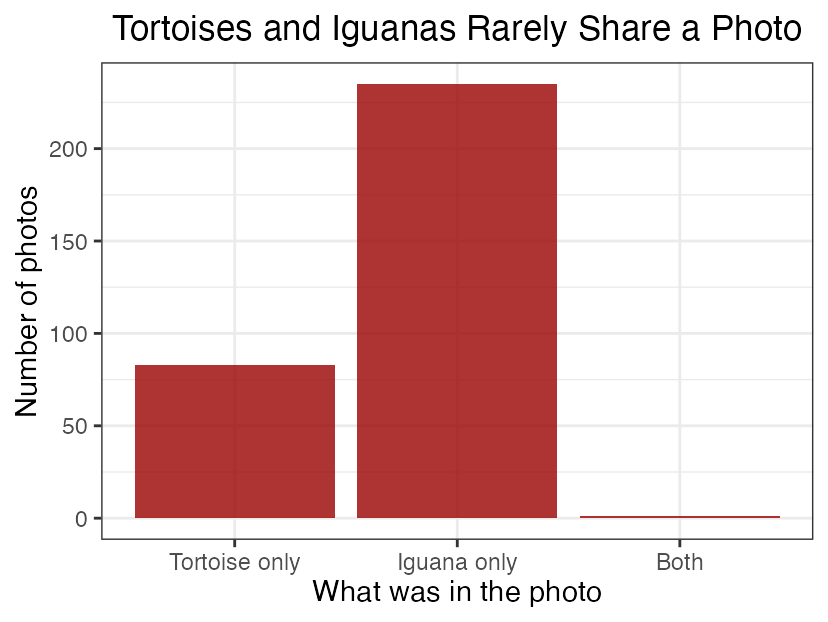
\includegraphics[width=0.3\linewidth,height=\textheight,keepaspectratio]{Imagesss/tortoises_iguanas_rare.png}

}

\caption{Bar chart showing how rarely tortoises and iguanas were
photographed together}

\end{figure}%

\subsubsection{Species by Camera Trap (Alluvial
Chart)}\label{species-by-camera-trap-alluvial-chart}

\begin{Shaded}
\begin{Highlighting}[]
\NormalTok{dffocal\_loc }\SpecialCharTok{\%\textgreater{}\%}
  \FunctionTok{count}\NormalTok{(species, camera\_trap\_name, }\AttributeTok{name =} \StringTok{"frequency"}\NormalTok{) }\SpecialCharTok{\%\textgreater{}\%}
  \FunctionTok{ggplot}\NormalTok{(}\FunctionTok{aes}\NormalTok{(}\AttributeTok{y =}\NormalTok{ frequency, }\AttributeTok{axis1 =}\NormalTok{ species, }\AttributeTok{axis2 =}\NormalTok{ camera\_trap\_name)) }\SpecialCharTok{+}
  \FunctionTok{geom\_alluvium}\NormalTok{(}\FunctionTok{aes}\NormalTok{(}\AttributeTok{fill =}\NormalTok{ species), }\AttributeTok{width =} \DecValTok{1}\SpecialCharTok{/}\DecValTok{6}\NormalTok{) }\SpecialCharTok{+}
  \FunctionTok{geom\_stratum}\NormalTok{(}\AttributeTok{alpha =} \FloatTok{0.5}\NormalTok{, }\AttributeTok{width =} \DecValTok{1}\SpecialCharTok{/}\DecValTok{6}\NormalTok{) }\SpecialCharTok{+}
  \FunctionTok{geom\_text}\NormalTok{(}\AttributeTok{stat =} \StringTok{"stratum"}\NormalTok{, }\AttributeTok{size =} \DecValTok{3}\NormalTok{, }\FunctionTok{aes}\NormalTok{(}\AttributeTok{label =} \FunctionTok{after\_stat}\NormalTok{(stratum))) }\SpecialCharTok{+}
  \FunctionTok{scale\_fill\_manual}\NormalTok{(}\AttributeTok{values =} \FunctionTok{c}\NormalTok{(}
    \StringTok{"\#9c0100"}\NormalTok{,}
    \StringTok{"\#ffcd01"}
\NormalTok{  )) }\SpecialCharTok{+}
  \FunctionTok{scale\_x\_discrete}\NormalTok{(}\AttributeTok{limits =} \FunctionTok{c}\NormalTok{(}\StringTok{"Species"}\NormalTok{, }\StringTok{"Camera trap"}\NormalTok{), }\AttributeTok{expand =} \FunctionTok{c}\NormalTok{(}\FloatTok{0.1}\NormalTok{, }\FloatTok{0.1}\NormalTok{)) }\SpecialCharTok{+}
  \FunctionTok{labs}\NormalTok{(}\AttributeTok{title =} \StringTok{"Which Camera Trap Each Species Was Detected"}\NormalTok{,}
       \AttributeTok{y =} \StringTok{"Number of detections"}\NormalTok{, }\AttributeTok{fill =} \StringTok{"Species"}\NormalTok{) }\SpecialCharTok{+}
  \FunctionTok{theme\_bw}\NormalTok{() }\SpecialCharTok{+}
  \FunctionTok{theme}\NormalTok{(}\AttributeTok{plot.title =} \FunctionTok{element\_text}\NormalTok{(}\AttributeTok{hjust =} \FloatTok{0.5}\NormalTok{))}

\FunctionTok{ggsave}\NormalTok{(}\AttributeTok{filename =} \StringTok{"../output/r\_analysis/SpeciesByCameraAlluvialPlot.png"}\NormalTok{, }\AttributeTok{width =} \DecValTok{10}\NormalTok{, }\AttributeTok{height =} \DecValTok{8}\NormalTok{, }\AttributeTok{dpi =} \DecValTok{300}\NormalTok{)}
\end{Highlighting}
\end{Shaded}

\begin{figure}[H]

{\centering 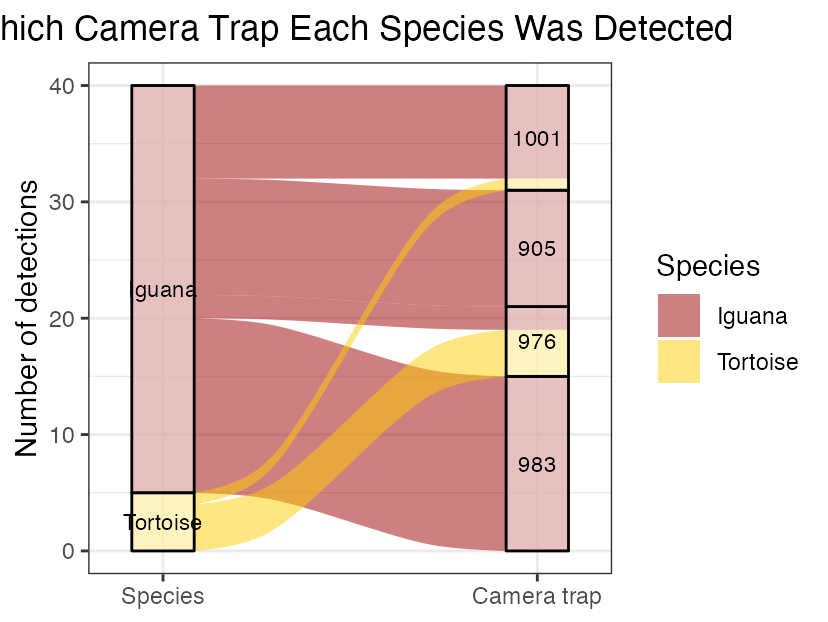
\includegraphics[width=0.3\linewidth,height=\textheight,keepaspectratio]{Imagesss/which_camera_trap.png}

}

\caption{Chart comparing where each species was detected across camera
sites}

\end{figure}%

\subsubsection{Activity by Time of Day, by
Camera}\label{activity-by-time-of-day-by-camera}

\begin{Shaded}
\begin{Highlighting}[]
\NormalTok{dffocal\_loc }\SpecialCharTok{\%\textgreater{}\%}
  \FunctionTok{count}\NormalTok{(camera\_trap\_name, time\_of\_day, species) }\SpecialCharTok{\%\textgreater{}\%}
  \FunctionTok{group\_by}\NormalTok{(camera\_trap\_name, species) }\SpecialCharTok{\%\textgreater{}\%}
  \FunctionTok{mutate}\NormalTok{(}
    \AttributeTok{total      =} \FunctionTok{sum}\NormalTok{(n),}
    \AttributeTok{proportion =}\NormalTok{ n }\SpecialCharTok{/}\NormalTok{ total,}
    \AttributeTok{se         =} \FunctionTok{sqrt}\NormalTok{(proportion }\SpecialCharTok{*}\NormalTok{ (}\DecValTok{1} \SpecialCharTok{{-}}\NormalTok{ proportion) }\SpecialCharTok{/}\NormalTok{ total)}
\NormalTok{  ) }\SpecialCharTok{\%\textgreater{}\%}
  \FunctionTok{ungroup}\NormalTok{() }\SpecialCharTok{\%\textgreater{}\%}
  \FunctionTok{ggplot}\NormalTok{(}\FunctionTok{aes}\NormalTok{(}\AttributeTok{x =}\NormalTok{ time\_of\_day, }\AttributeTok{y =}\NormalTok{ proportion, }\AttributeTok{fill =}\NormalTok{ species)) }\SpecialCharTok{+}
  \FunctionTok{geom\_col}\NormalTok{(}\AttributeTok{position =} \FunctionTok{position\_dodge}\NormalTok{(}\AttributeTok{width =} \FloatTok{0.9}\NormalTok{)) }\SpecialCharTok{+}
  \FunctionTok{geom\_errorbar}\NormalTok{(}\FunctionTok{aes}\NormalTok{(}\AttributeTok{ymin =} \FunctionTok{pmax}\NormalTok{(proportion }\SpecialCharTok{{-}}\NormalTok{ se, }\DecValTok{0}\NormalTok{), }\AttributeTok{ymax =}\NormalTok{ proportion }\SpecialCharTok{+}\NormalTok{ se),}
                \AttributeTok{position =} \FunctionTok{position\_dodge}\NormalTok{(}\AttributeTok{width =} \FloatTok{0.9}\NormalTok{), }\AttributeTok{width =} \FloatTok{0.2}\NormalTok{) }\SpecialCharTok{+}
  \FunctionTok{scale\_fill\_manual}\NormalTok{(}\AttributeTok{values =} \FunctionTok{c}\NormalTok{(}\StringTok{"\#9a0101"}\NormalTok{, }\StringTok{"\#ffcd01"}\NormalTok{)) }\SpecialCharTok{+}
  \FunctionTok{labs}\NormalTok{(}\AttributeTok{title =} \StringTok{"Tortoise and Iguana Activity Peaks at Different Times of Day"}\NormalTok{,}
       \AttributeTok{x =} \StringTok{"Time of day"}\NormalTok{, }\AttributeTok{y =} \StringTok{"Proportion of that species\textquotesingle{} detections"}\NormalTok{,}
       \AttributeTok{fill =} \StringTok{"Species"}\NormalTok{) }\SpecialCharTok{+}
  \FunctionTok{theme\_bw}\NormalTok{() }\SpecialCharTok{+}
  \FunctionTok{theme}\NormalTok{(}\AttributeTok{plot.title =} \FunctionTok{element\_text}\NormalTok{(}\AttributeTok{hjust =} \FloatTok{0.5}\NormalTok{)) }\SpecialCharTok{+}
  \FunctionTok{facet\_wrap}\NormalTok{(}\SpecialCharTok{\textasciitilde{}}\NormalTok{camera\_trap\_name)}

\FunctionTok{ggsave}\NormalTok{(}\AttributeTok{filename =} \StringTok{"../output/r\_analysis/TimeOfDayByCameraPlot.png"}\NormalTok{, }\AttributeTok{width =} \DecValTok{19}\NormalTok{, }\AttributeTok{height =} \DecValTok{8}\NormalTok{, }\AttributeTok{dpi =} \DecValTok{300}\NormalTok{)}
\end{Highlighting}
\end{Shaded}

\begin{figure}[H]

{\centering 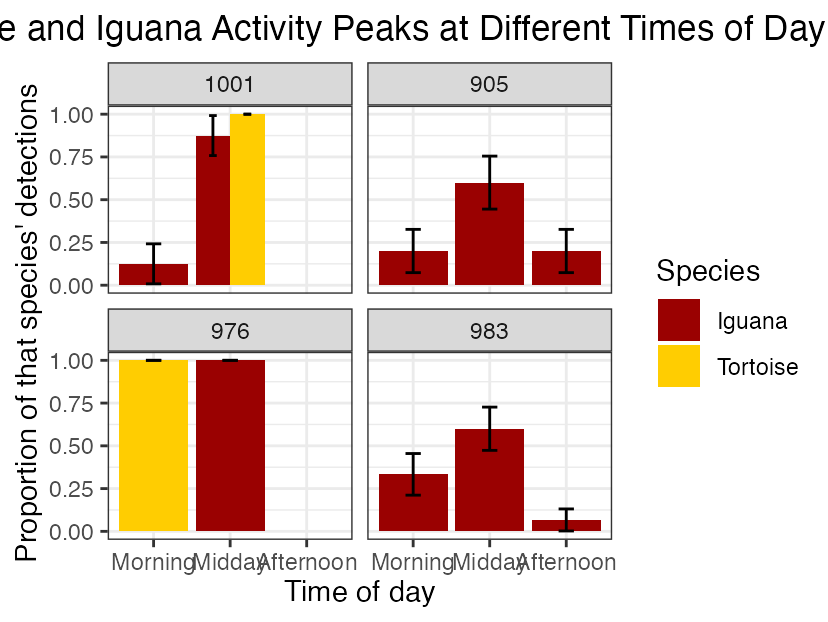
\includegraphics[width=0.3\linewidth,height=\textheight,keepaspectratio]{Imagesss/peak_activity_times.png}

}

\caption{Chart comparing each species' activity levels across different
times of day, broken down by camera trap site}

\end{figure}%

\subsubsection{Hourly Detection Pattern}\label{hourly-detection-pattern}

\begin{Shaded}
\begin{Highlighting}[]
\NormalTok{dffocal }\SpecialCharTok{\%\textgreater{}\%}
  \FunctionTok{ggplot}\NormalTok{(}\FunctionTok{aes}\NormalTok{(}\AttributeTok{x =}\NormalTok{ hour, }\AttributeTok{fill =}\NormalTok{ species)) }\SpecialCharTok{+}
  \FunctionTok{geom\_histogram}\NormalTok{(}\AttributeTok{binwidth =} \DecValTok{1}\NormalTok{, }\AttributeTok{position =} \StringTok{"identity"}\NormalTok{, }\AttributeTok{alpha =} \FloatTok{0.5}\NormalTok{) }\SpecialCharTok{+}
  \FunctionTok{labs}\NormalTok{(}\AttributeTok{title =} \StringTok{"Hourly Detection Pattern by Species"}\NormalTok{,}
       \AttributeTok{x =} \StringTok{"Hour of day"}\NormalTok{, }\AttributeTok{y =} \StringTok{"Number of detections"}\NormalTok{, }\AttributeTok{fill =} \StringTok{"Species"}\NormalTok{) }\SpecialCharTok{+}
  \FunctionTok{scale\_fill\_manual}\NormalTok{(}\AttributeTok{values =} \FunctionTok{c}\NormalTok{(}\StringTok{"\#9a0101"}\NormalTok{, }\StringTok{"\#ffcd01"}\NormalTok{)) }\SpecialCharTok{+}
  \FunctionTok{theme\_bw}\NormalTok{() }\SpecialCharTok{+}
  \FunctionTok{theme}\NormalTok{(}\AttributeTok{plot.title =} \FunctionTok{element\_text}\NormalTok{(}\AttributeTok{hjust =} \FloatTok{0.5}\NormalTok{))}

\FunctionTok{ggsave}\NormalTok{(}\AttributeTok{filename =} \StringTok{"../output/r\_analysis/HourlyActivityPlot.png"}\NormalTok{, }\AttributeTok{width =} \DecValTok{10}\NormalTok{, }\AttributeTok{height =} \DecValTok{8}\NormalTok{, }\AttributeTok{dpi =} \DecValTok{300}\NormalTok{)}
\end{Highlighting}
\end{Shaded}

\begin{figure}[H]

{\centering 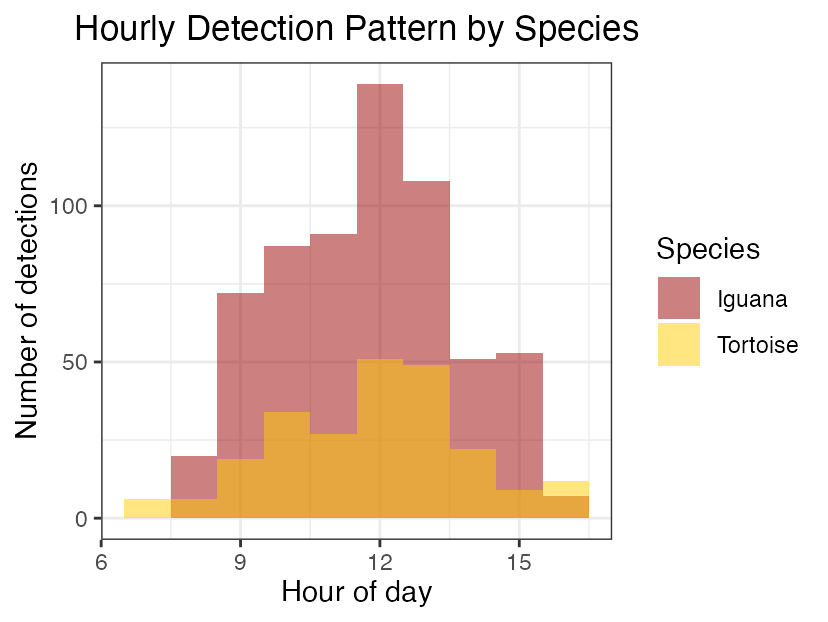
\includegraphics[width=0.3\linewidth,height=\textheight,keepaspectratio]{Imagesss/hourly_detection_by_species.png}

}

\caption{Chart showing the raw hourly detection pattern for each species
across the day}

\end{figure}%

\subsection{Results Summary}\label{results-summary}

Out of the images I classified, tortoises and iguanas were rarely
photographed together, appearing in the same frame in less than 1\% of
images. Both species were active during similar times of day, with
detections peaking around midday for each, yet they tended to favor
different camera trap sites overall. Together, these results suggest the
two species may coexist by avoiding direct contact at a spatial scale,
rather than by separating according to time of day. For my full research
poster and discussion of these findings,
\href{https://postimg.cc/fkHGkFGB}{see here}.

\begin{center}
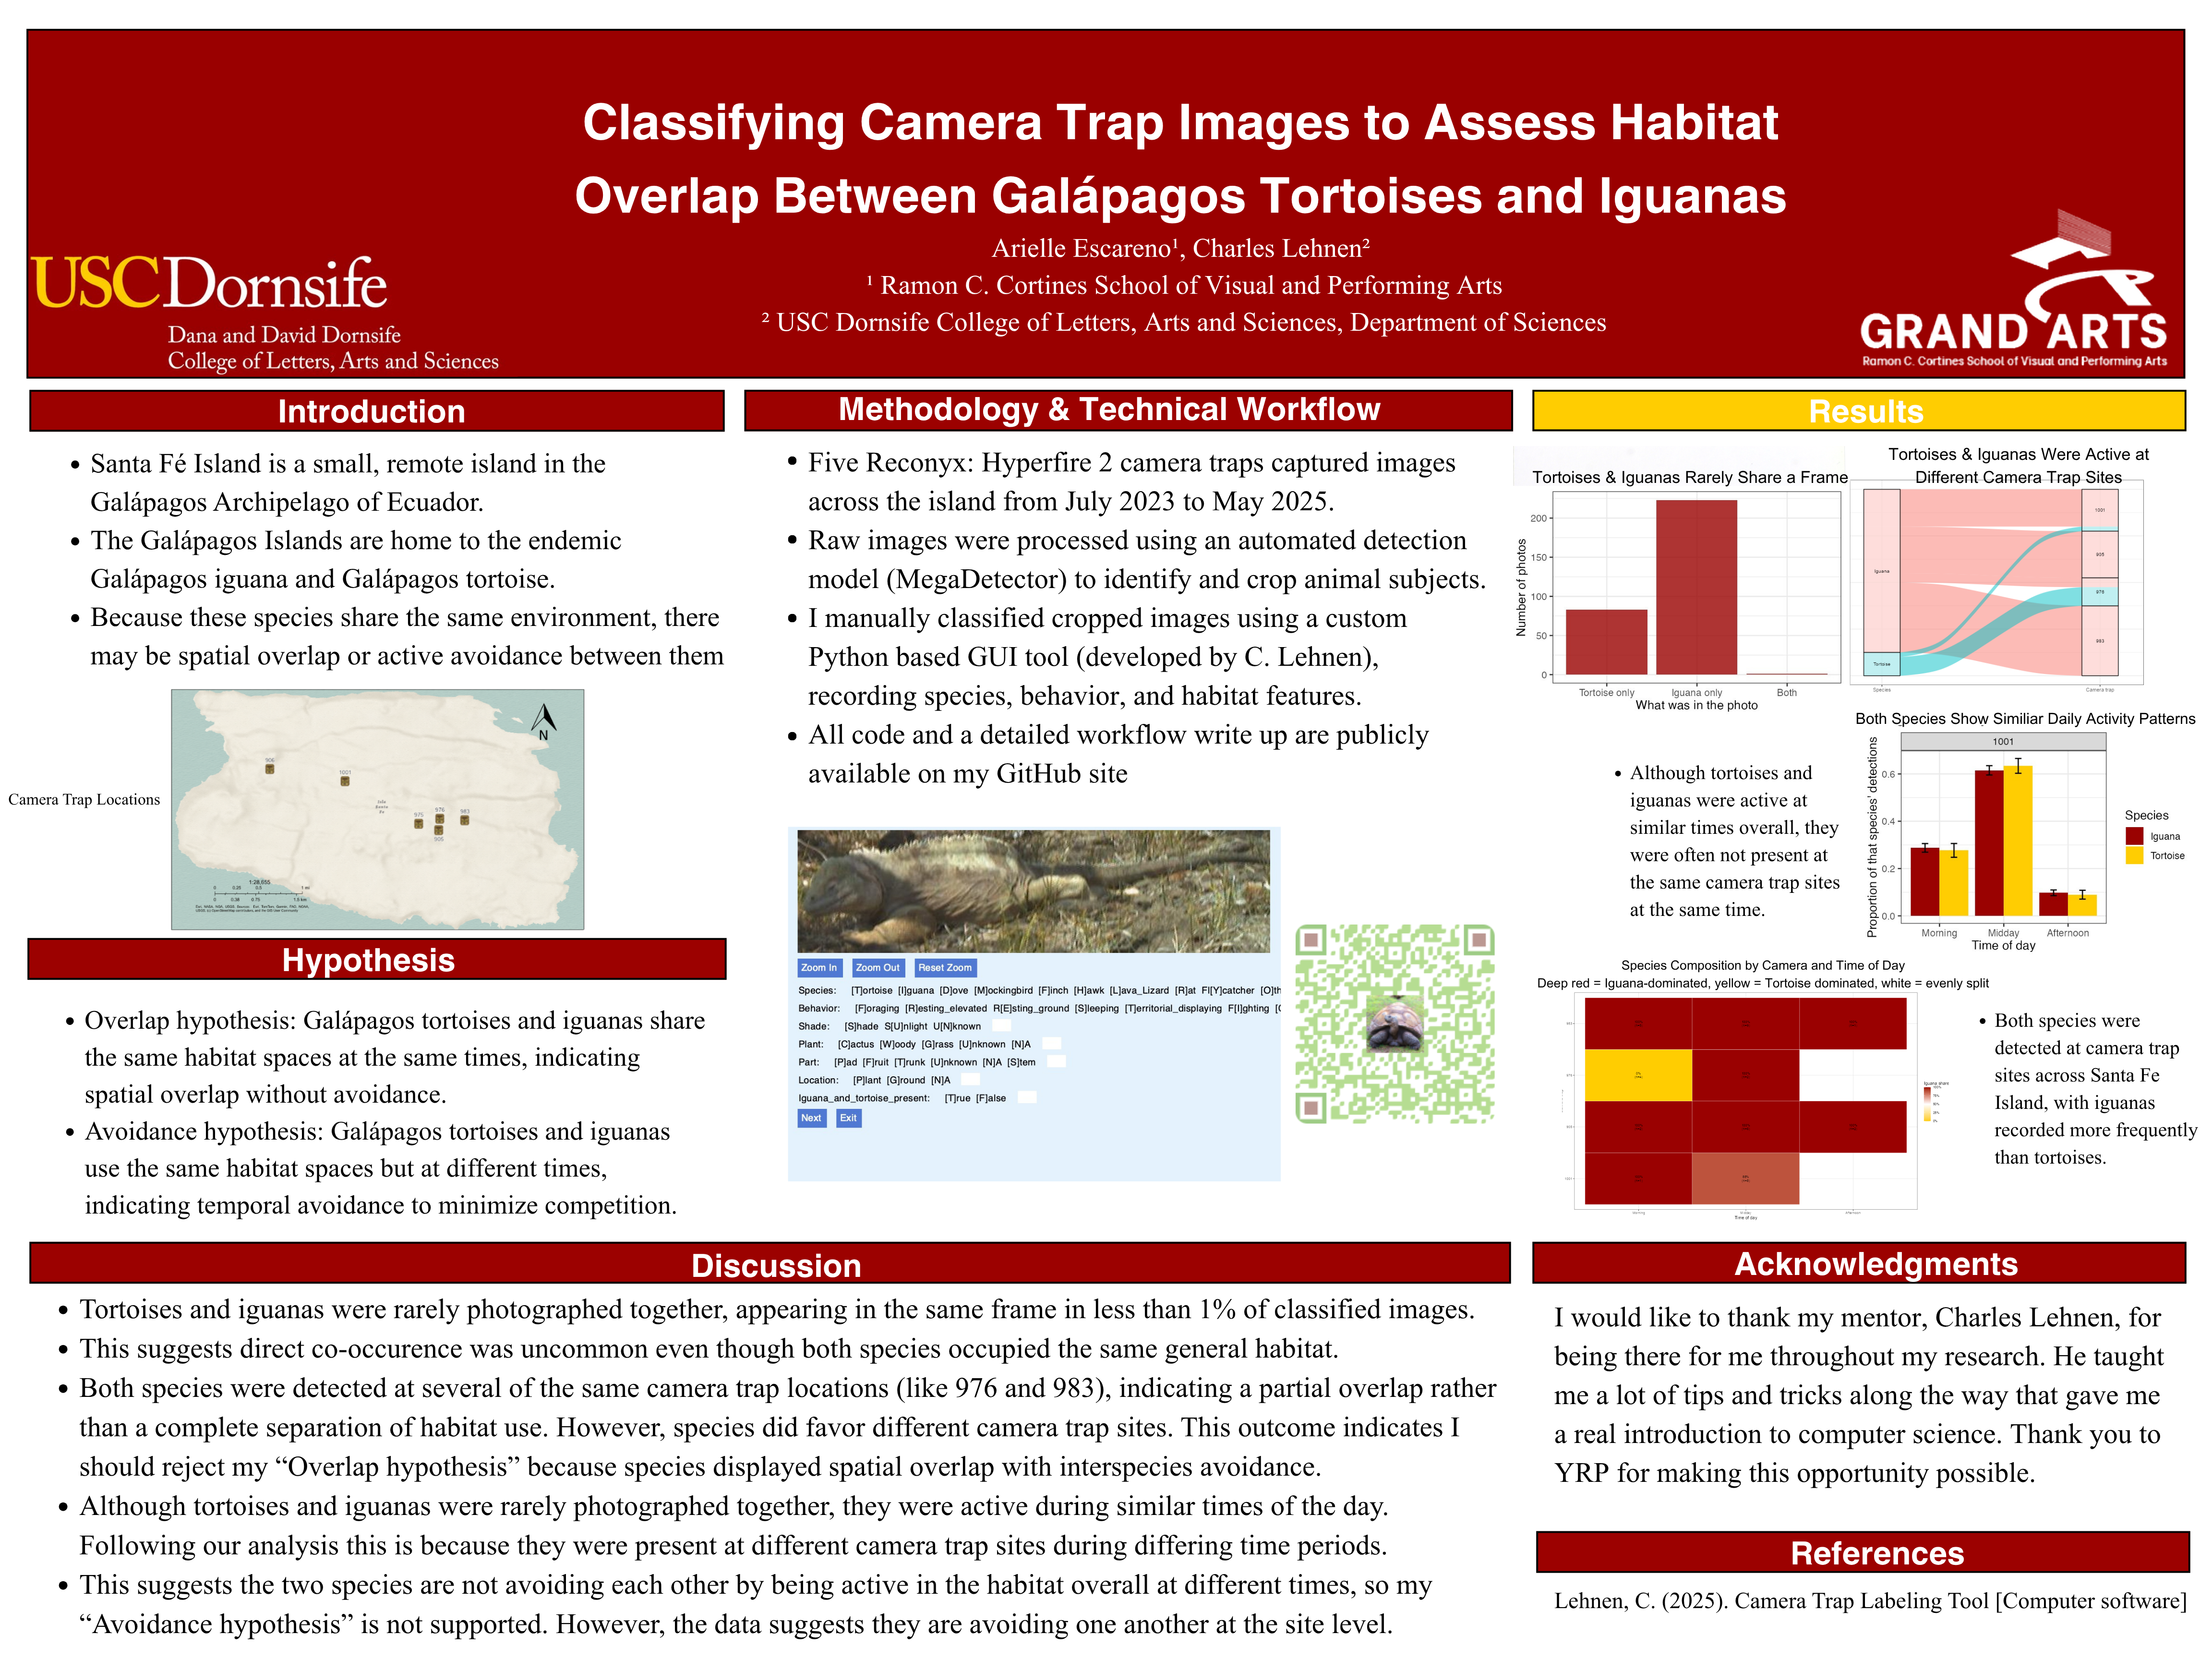
\includegraphics[width=9.04167in,height=\textheight,keepaspectratio]{images/paste-3.png}
\end{center}

\subsection{Discussion}\label{discussion}

Tortoises and iguanas were rarely photographed together, appearing in
the same frame in less than 1\% of classified images.

\begin{itemize}
\tightlist
\item
  This suggests direct co-occurrence was uncommon even though both
  species occupied the same general habitat.
\item
  Both species were detected at several of the same camera trap
  locations (like 976 and 983), indicating a partial overlap rather than
  a complete separation of habitat use. However, species did favor
  different camera trap sites. This outcome indicates I should reject my
  ``Overlap hypothesis'' because species displayed spatial overlap with
  interspecies avoidance.
\item
  Although tortoises and iguanas were rarely photographed together, they
  were active during similar times of the day. Following our analysis
  this is because they were present at different camera trap sites
  during differing time periods.
\item
  This suggests the two species are not avoiding each other by being
  active in the habitat overall at different times, so my ``Avoidance
  hypothesis'' is not supported. However, the data suggests they are
  avoiding one another at the site level.
\end{itemize}

\subsection{Reflections}\label{reflections}

Overall, having the opportunity to work one on one with someone who's an
expert in this field has been an amazing experience. Although I'm not
necessarily interested in biological sciences, I am interested in
computer science, so this project gave me hands-on skills I can directly
apply to future computer science work. Beyond the bigger technical
skills, I picked up a lot of small, practical tricks along the way that
made me faster and more comfortable working in the terminal. Using the
up arrow to re-run a command I'd already typed instead of retyping it
saved some time. I also learned the importance of committing my changes
regularly as I worked, so that my progress was always saved and
recoverable. I also learned firsthand how research doesn't always go the
way you expect. My original hypotheses predicted either full habitat
overlap or a clear pattern of time-based avoidance between species, but
my actual data showed something more nuanced than either option, which
pushed me to think more carefully about what my results really meant
instead of forcing them into a simple yes or no conclusion.




\end{document}
